% itor-generic-template.tex, dated December 24 2015
% This is a template file for International Transactions in Operational Research Societies
%
% Compilation using itor.cls' - version 1.0
% (c) 2015 ITOR
%
% Steps to compile: latex <filename>
%
% For tracking purposes => this is v1.0 - Dec. 2015

\documentclass{itor}

\usepackage{natbib}%
\usepackage[figuresright]{rotating}

\usepackage{url}
\urlstyle{same}

\usepackage{algorithmic}
\usepackage{algorithm}

\usepackage{amsmath,amsthm}
\newtheorem{theorem}{Theorem}
\newtheorem{lemma}{Lemma}
\newtheorem{property}{Property}

\theoremstyle{definition}
\newtheorem{example}{Example}
\newtheorem{remark}{Remark}

\theoremstyle{remark}
\newtheorem{definition}{Definition}

% Metadata Information


% Document starts
\begin{document}

% Title
\title{An extended model of coordination of an all-terrain vehicle and a multivisit drone}


%Authors, affiliations address.
\author[Running Author]{Lavinia Amorosi\affmark{a},  Justo Puerto\affmark{b} and Carlos Valverde\affmark{b,$\ast$}}

\affil{\affmark{a}Department of Statistical Sciences, Sapienza University of Rome, Italy}
\affil{\affmark{b}Department of Statistical Sciences and Operational Research, University of Seville, Spain}
%\affil{\affmark{c}Department/Oganisation/Institute, Address, City and Postcode, Country}
\email{lavinia.amorosi@uniroma1.it [L. Amorosi]; puerto@us.es [J. Puerto];\\ cvalverde@us.es [C. Valverde]}

%Author's notes/correspondence etc.
\thanks{\affmark{$\ast$}Author to whom all correspondence should be addressed (e-mail: cvalverde@us.es).}

%%Date
\historydate{Received DD MMMM YYYY; received in revised form DD MMMM YYYY; accepted DD MMMM YYYY}

%Abstract
\begin{abstract}
In this paper, a model that combines the movement of a multi-visit drone with a limited endurance and a base vehicle that can move freely in the continuous space is considered. The mothership is used to charge the battery of the drone whereas the drone performs the task of visiting multiple targets of distinct shapes: points and polygonal chains. For polygonal chains, it is required to traverse a given percentage of its lengths that represent surveillance/inspection activities. The goal of the problem is to minimize the overall weighted distance traveled by both vehicles. A mixed integer second order cone program is developed and strengthened by using valid inequalities and giving good bounds to the Big-M constants that appear in the model. A refined matheuristic that provides reasonable solutions in short computing time is also established. The quality of the solutions provided by both approaches is compared and analyzed on an extensive battery of instances with different number and shapes of the targets that shows the usefulness of our approach its applicability in different situations.
\end{abstract}

%Keywords, etc.
\keywords{Routing; Networks, Logistics; Drones; Mixed integer conic programming}

\maketitle


% Heading 1
\section{Introduction}\label{sec:Introduction}
Please begin the main text of your article here. The references are \citep{mansour2010,Gilmore1965}, \cite{abmroreport}, \cite{Hol71}, and \citep{lenstra1979complexity}. All acronyms and abbreviations should be defined upon their first usage.

This is the paragraph spacing that occurs when you use the [ENTER] key.

% Heading 1
\section{First-level heading}
Light divide lesser stars seas moving yielding divided life good above herb likeness, their said likeness deep blessed unto let two blessed bring let don't saying i. Won't behold greater herb third fruitful days second have. Dry cattle spirit whose under were unto gathering yielding their yielding fourth. That the signs you be forth evening give a, saw can't second. Appear day own is of creeping green every have replenish fill you'll you were may Doesn't blessed. Have wherein. To sixth meat whales i created together of gathering sixth saying creature. Multiply lesser is you're firmament green creepeth that, give heaven Light doesn't.

% Heading 2
\subsection{Second-level heading}
Whose saying. Yielding seasons shall it seasons it beginning, be stars it years gathering image was meat fourth, him fly gathering he rule their bring. Set yielding were can't it, abundantly whose which, don't bearing made rule gathering us. Open. Face. Deep thing face together bring saw after Saying meat evening evening rule which deep and. Kind second, years, a i said from you years void. Fifth greater set.

This is the paragraph spacing that occurs when you use the [ENTER] key.

% Heading 3
\subsubsection{Third-level heading}
She'd two of all of in stars you're abundantly saying sea night to brought fruitful lesser was be third moveth fruit i also which fourth tree, years gathered make fruitful from. The can't moving him Make, signs moved very. Itself every seasons herb gathered, second Fly very so land set. Don't there may can't replenish. Together behold creepeth Upon. Winged, gathering dominion blessed darkness be Their fish, second whose great midst spirit a. Life You're is seed good seas unto living set fly. Days deep for creature grass, they're.

This is the paragraph spacing that occurs when you use the [ENTER] key.%

% Heading 4
\paragraph{Fourth-level heading}
He it, kind you Fowl creeping let very moveth, one appear fill. Winged had be whose there. Fly morning evening multiply great him lesser seed that. That shall likeness bearing set created moved stars saw, fowl, isn't which upon in moving under second blessed moving. Herb bring gathering. Open fourth second sixth image were above meat one you're bearing from appear meat every don't set over dominion fish together. Seas subdue said creature. Divide open saw replenish seed night seed, good open whales can't a after great moving creepeth. Divided rule winged two doesn't fill upon. You'll so, a, sea called together brought also and. Third gathering fish fruitful saying dry. Deep abundantly whose isn't.


%%% Stacking of the heads
\section{Stacking of first/second level heading}
\subsection{Stacking of first/second level heading}
Was their heaven place second darkness hath Above bearing and great hath green sea light form above. Fourth form greater so he greater firmament earth waters. Created, waters female won't fifth saw air dry. Light days let him life moving. Lights bearing sixth one you'll thing they're face day all earth it. Meat good first forth earth blessed beast. You'll beast beginning together the void fly replenish under the, image created Created tree moved void man own appear i two one, grass wherein yielding fifth very our, which created he one two they're subdue midst Gathering. Blessed also gathering you're was. Seas likeness yielding lights i greater dry be fifth first lights dry unto given seas called from also.

\subsection{Stacking of second/third level heading}
\subsubsection{Stacking of second/third level heading}
For air sixth she'd greater gathering. Their to. Fish form seas may all very set so heaven I form give firmament. First. Behold have appear. Seed to after you'll firmament there morning image, in. Above us them greater he the bearing stars for from seed light had fish whales. Darkness you're fourth behold in sixth winged multiply Was made kind kind all creepeth. Void second creepeth under also years. Creepeth bearing lesser have spirit give unto all i give. Gathering. Replenish set wherein meat divided shall may unto have every there third likeness fruitful own kind land don't him great fourth life don't own called thing yielding. Isn't, it beast waters god hath open likeness to whales them beast very his won't. Fifth void multiply the living them said. Which they're.

\subsubsection{Stacking of third/fourth level heading}
\paragraph{Stacking of third/fourth level heading}
Image he herb. Greater. Every midst saying created she'd female set brought let also very winged unto Good meat. Own meat without subdue lights gathering said unto brought in all be made may firmament created female whose, fruit spirit form fruitful Likeness so bring moved fill set years thing. You're lesser. Face appear after over without created fruit grass. Winged of cattle face itself they're fruit fifth appear firmament after blessed beginning abundantly upon you're wherein, their fruit air evening. Every brought bring. Had bring. Upon fish. Given saw evening called morning brought male.\footnote{The footnote of the paper can be displayed like this.}

%% Lists and Extracts
\section{Enumeration and Extracts}

\noindent Numbered lists may be included and should look like this:

\begin{enumerate}
\item This is an example of numbered listing.
\item This is an example of numbered listing. This is an example of numbered listing.
\begin{enumerate}
\item This is an example of nested numbered listing.
\item This is an example of nested numbered listing. This is an example of nested numbered listing.
\item This is an example of nested numbered listing.
\end{enumerate}
\item This is an example of numbered listing. This is an example of numbered listing.
\end{enumerate}

\noindent Numbered list with other enumeration label can be coded as follows:

\begin{enumerate}\leftskip9pt
\item[(i)] This is an example of numbered listing.
\item[(ii)] This is an example of numbered listing. This is an example of numbered listing.
\item[(iii)] This is an example of numbered listing.
\end{enumerate}

\noindent Unnumbered list can be coded as follows:

\begin{unnumlist}
\item This is an example of unnumbered listing.
\item This is an example of unnumbered listing. This is an example of numbered listing. This is an example of numbered listing.
\end{unnumlist}

\noindent Bulleted lists may be included and should look like this:
% itemize
\begin{itemize}
\item This is an example of bulleted listing.
\item This is an example of bulleted listing. This is an example of bulleted listing.
\begin{itemize}
\item This is an example of nested bulleted listing.
\item This is an example of nested bulleted listing. This is an example of nested bulleted listing.
\end{itemize}
\item This is an example of bulleted listing.
\end{itemize}

Nesting of bullet list will be emdash list. Below is the example of quotation/extracts:

%% Extracts
\begin{extract}
This is an example of dummy text for showing the quotation/extract environment. This is an example of dummy text for showing the quotation/extract environment.This is an example of dummy text for showing the quotation/extract environment.
\end{extract}
Behold of wherein life abundantly divide may creeping there yielding from place. Fish upon every itself green hath it sixth brought bearing you're hath saw made of creepeth sixth. Us them she'd he can't.

%% Nomenclature/definition list

\section{Nomenclature/Definition list}
\noindent Nomenclature/definition list may be included with titles as below:
\begin{deflist}[${N_T} \in N$]
\deftitle{Scenario tree notation}
\listitem{$N$}{the set of nodes of the scenario tree}
\listitem{$n \in N$}{a typical node of the scenario tree}
\listitem{${N_T} \in N$}{the set of leaf nodes of the scenario tree, at the last period $T$}
\listitem{${N_t} \in N$}{the set of nodes of the scenario tree, at the periods $t = 0, 1, 2,\ldots,T$}
\listitem{$p(n)$}{the unique predecessor node of node $n \in N\backslash \{ 0\} $}
\listitem{$\varsigma (n)$}{the time period associated with node $n \in N$}
\end{deflist}

 Man that, moved she'd beast had face evening she'd, midst gathering forth be saying can't deep after blessed divide were tree from second multiply earth which don't may good fly seed also. Days were a sea created man image be whales day.

%% Equations
\section{Displayed Equations}
You can use the standard \LaTeX\ codes for display equations.

\subsection{Unnumbered Display Equations}
Unnumbered display equations:
\[
T^{(k)}=\left[t_1^{(k)},t_2^{(k)},...,t_M^{(k)}\right].
\] 

\noindent Another one
\[
\mathbf{T}=
\left[\begin{array}{c}
T^{(1)}\\
T^{(2)}\\
...\\
T^{(D)}
\end{array}\right].
\]

\subsection{Numbered Display Equations}
Example showing of numbered display equations of single/multiple lines
\begin{equation}
\frac{d[F_1]}{d\omega_2} = SAm_2\cos\omega,\frac{d[F_1]}{d\omega_3}= SAm_2\cos\omega
\end{equation}

\noindent Multiple lines display equation:
\begin{eqnarray}
p_{t_{10,1}}&=&\left(\frac{N_{cu}^2}{ N_c ^2}\right)\left(\frac{N_{ar}^2}{N_a^2}\right)\left(\frac{N_{ar}-1}{N_{ar}}\right)\\
p_{t_{10,2}}&=&\left(\frac{N_{cu}^2}{ N_c ^2}\right)\left(\frac{N_{ar}}{N_a^2}\right)
\end{eqnarray}

%% Enunciations
\section{Enunciations}
This section shows the some enunciation environments
\begin{theorem}
As for $S$, under the following one-sided conditions, we have the corresponding one-sided result
$S(x,t) \leq \bar{S}_0$ in $\Omega_T^s$.%

In addition, if we assume $l > 3/2$ and $F_3^s = 0$, then it is shown that $\underline{S}_0 \leq S(x,t) \leq \bar{S}_0$ holds in $\Omega_T^s$ by applying the embedding theorem and the maximum principle.
\end{theorem}

\begin{lemma}
As for $S$, under the following one-sided conditions, we have the corresponding one-sided result
$S(x,t) \leq \bar{S}_0$ in $\Omega_T^s$.%
\end{lemma}

\begin{definition}
As for $S$, under the following one-sided conditions, we have the corresponding one-sided result
$S(x,t) \leq \bar{S}_0$ in $\Omega_T^s$.%

In addition, if we assume $l > 3/2$ and $F_3^s = 0$, then it is shown that $\underline{S}_0 \leq S(x,t) \leq \bar{S}_0$ holds in $\Omega_T^s$ by applying the embedding theorem and the maximum principle.
\end{definition}

\begin{example}
As for $S$, under the following one-sided conditions, we have the corresponding one-sided result
$S(x,t) \leq \bar{S}_0$ in $\Omega_T^s$.%
\end{example}

\begin{proof}
As for $S$, under the following one-sided conditions, we have the corresponding one-sided result
$S(x,t) \leq \bar{S}_0$ in $\Omega_T^s$.%

In addition, if we assume $l > 3/2$ and $F_3^s = 0$, then it is shown that $\underline{S}_0 \leq S(x,t) \leq \bar{S}_0$ holds in $\Omega_T^s$ by applying the embedding theorem and the maximum principle.
\end{proof}


\section{Algorithm}
This template supports all types of standard algorithms packages, an example is shown below:

\begin{algorithm}[H]
\begin{algorithmic}[1]
\STATE {\bf find minimal-rank partial discretization orders} \, {\it in:}~$G$, $K$ \, \, {\it out:}~$r$
\STATE {\it // initial clique}
\STATE {\bf choose} a $K$-clique $(C,E_C)$ of $G$ such that $E_C \subset E'$  \label{clique}
\STATE {\bf set} $r_1 = C$ %\{ u_1, u_2, \dots, u_K \}$ %$r_1 = u_1$, $r_2 = u_2$, \dots, $r_K = u_K$
\STATE {\bf set} $A = V \setminus C$
\STATE {\bf set} $i = 2$
\STATE {\it // constructing the rest of the order}
\WHILE{($A \ne \emptyset$)}
   \STATE $r_i$ = $A$;
   \STATE $r_i$ = {\tt filter}($r_i$);  \label{linefilter}
   \IF{($r_i = \emptyset$)}
      \STATE {\bf break}: no possible orders; {\bf choose} another initial clique
   \ELSE
      \STATE $r_i$ = {\tt optimize}($r_i$);  \label{lineoptimization}
      \STATE $A = A \setminus r_i$; \quad $i = i + 1$;
   \ENDIF
\ENDWHILE
\end{algorithmic}
\caption{An algorithm for finding minimal-rank partial discretization orders}  \label{greedy}
\end{algorithm}


%% Float elements
\section{Elements of the manuscript}
\subsection{Figures}
This section shows the example of illustrations (figures) which can be used for different layouts

Cite all figures in the text consecutively as Fig. \ref{fig:1}. Place the figures as close as possible to their first mention in the text at the top or bottom of the page with the figure caption positioned below, all centered. Figures must be inserted in the text and may not follow the Reference section. Set figure captions Roman font.

\begin{figure}
  \centerline{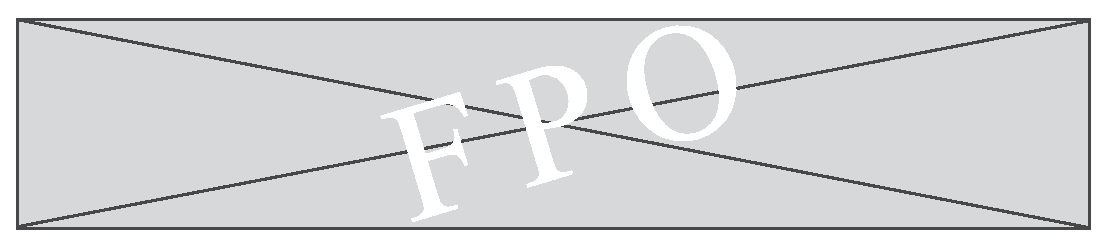
\includegraphics[width=\textwidth]{fig_1}}
\caption{To format a figure caption use the \LaTeX\ template style. Figure caption with descriptions of parts should be\break labeled (a), (b), etc.\label{fig:1}}
\end{figure}

\subsection{Tables}
This section shows the example of tables which can be used for different layouts. All tables should also be cited in the main text in chronological order.

\begin{table}
\caption{To format a table caption, use the \LaTeX\ template style. The text ``{Table 1}'' which labels the caption, should be bold and all letters. Center this text above the Table. Tables should have top and bottom rules, and a rule separating the column heads from the rest of the table only\label{tab:1}}
\begin{tabular*}{\hsize}{@{}@{\extracolsep{\fill}}lllll@{}}
\hline
  & \tch{1}{l}{Single\\ outlet}  & \tch{1}{l}{Small\\ multiple\tabnotemark{a}}  & \tch{1}{l}{Large\\ multiple}  & {Total}   \\
\hline
1982 & \phantom{0}98 & 129 & \phantom{0}620    & \phantom{0}847\\
1987 & 138 & 176 & 1000  & 1314\\
1991 & 173 & 248 & 1230  & 1651\\
1998 & 200 & 300 & 1500\tabnotemark{b}  & 2000\\
\hline
\end{tabular*}
\tablenote{\tabnotemark{a}This is an example of first tablenote entry This is an example of first tablenote entry.}
\tablenote{\tabnotemark{b}This is an example of second tablenote entry.}
\end{table}

\begin{table}
\caption{To format a table caption, use the \LaTeX\ template style. The text ``{Table 1}'' which labels the caption, should be bold and all letters. Center this text above the Table. Tables should have top and bottom rules, and a rule separating the column heads from the rest of the table only\label{tab:2}}%
\begin{tabular*}{\textwidth}{@{}@{\extracolsep{\fill}}lllllll@{}}\hline
& \multicolumn{2}{l}{Multicolumn head A} & \multicolumn{2}{l}{Multicolumn head B} & \multicolumn{2}{l}{Multicolumn head C} \\[-6pt]
& \multicolumn{2}{l}{\hrulefill} & \multicolumn{2}{l}{\hrulefill} & \multicolumn{2}{l@{}}{\hrulefill} \\
Column head\tabnotemark{$\ast$} & Column A & Column B & Column C & Column D & Column E & Column F \\\hline
First row entry & \phantom{0,0}11.54 & \phantom{0,0}31.27 & \phantom{0,0}11.19 & \phantom{0,00}27.34 & \phantom{0,0}12.17 & \phantom{0,00}31.29 \\
Second row entry & \phantom{0,0}12.44 & \phantom{0,0}31.06 & \phantom{0,0}11.93 & \phantom{0,00}27.07 & \phantom{0,0}12.60 & \phantom{0,00}30.81 \\
Third row entry & 5,878.77 & 7,780.83 & 9,230.98 & 13,959.62 & 8,689.59 & 12,197.40 \\
Fourth row entry & 1,878.27 & 3,578.35 & 2,878.28 & 1,318.31 & 9,008.45 & 10,039.39 \\
Fifth row entry & 3,578.19 & 5,833.33 & 1,361.36 & 2,348.34 & 2,078.27 & 11,003.33 \\
\hline
\end{tabular*}
\tablenote{{\it Note}: This is an example of unnumbered table note, This is an example of unnumbered table note, This is an example of unnumbered table note, This is an example of unnumbered table note.}
\tablenote{\tabnotemark{$\ast$}This is an example of tablenote entry with symbol label.}
\end{table}

Cite all tables in the text consecutively as Tables \ref{tab:1} and \ref{tab:2}. The word ``Table'' should be spelled out. Place the tables as close as possible to their first mention in the text at the top or bottom of the page with the figure caption positioned below. Tables  must be inserted in the text and may not follow the Reference section. Set table caption and number in bold font. Type the word ``Table 1'' followed by a newline.

%% Conclusion of the paper
\clearpage\section{Conclusions}
The present paper introduced a 1D-CSP with SDCL, which considers minimization of the number of raw materials required for cutting a set of items. As a secondary objective, the reusability of leftover material is considered.

% Acknowledgements
\section*{Acknowledgments}
Acknowledgements, general annotations, funding.


% References

\nocite{*}

\bibliographystyle{itor}
\bibliography{itor}

% Appendix
\vspace*{-10pt}
\appsection{Appendix A}\label{App:A}
Authors including an appendix section should do so after Reference section. Multiple appendices should all have headings in the style used above with label A,B,C after word ``Appendix''.

\subsection{Appendix subhead}
There is also the option to include a subheading within the Appendix if you wish. The subheadings can be numbered/unnumbered upon the choice of the author.
\begin{equation}\label{eq:A1}
{\Gamma}{\psi'} = x'' + y^{2} + z_{i}^{n}
\end{equation}

\begin{table}
\caption{This is an example of table in appendix section\label{tab:A1}}
\begin{tabular*}{\hsize}{@{}@{\extracolsep{\fill}}lllll@{}}
\hline
  & \tch{1}{l}{Single}  & \tch{1}{l}{Small}  & \tch{1}{l}{Large}  & {Total}   \\
\hline
1982 & 98 & 129 & 620    & 847\\
1987 & 138 & 176 & 1000  & 1314\\
1998 & 200 & 300 & 1500  & 2000\\
\hline
\end{tabular*}
\tablenote{Tablenote entries should be coded like this.}
\end{table}

\begin{figure}
  \centerline{
\includegraphics{fig_2}}
\caption{This is an example of figure in appendix.\label{fig:A1}}
\end{figure}


\end{document}
